\documentclass{AeroStructure-ERJohnson}
\input crosslink.tex

%\usepackage{showframe}
\def\ShowFrameLinethickness{0.125pt}

\def\harp#1{\smash{\mathord{\buildrel{\lower3pt\hbox{$\scriptscriptstyle\rightharpoonup$}}\over{#1}}}}

\myexternaldocument{App_4P}
\myexternaldocument{Ch01_4P}
\myexternaldocument{Ch02_4P}
\myexternaldocument{Ch03_4P}
\myexternaldocument{Ch04_4P}
\myexternaldocument{Ch05_4P}
\myexternaldocument{Ch06_4P}
\myexternaldocument{Ch07_4P}
\myexternaldocument{Ch08_4P}
\myexternaldocument{Ch09_4P}
\myexternaldocument{Ch10_4P}
\myexternaldocument{Ch11_4P}
\myexternaldocument{Ch12_4P}
\myexternaldocument{Ch13_4P}
%\myexternaldocument{Ch14_4P}
\myexternaldocument{Ch15_4P}
\myexternaldocument{Ch16_4P}
\myexternaldocument{Ch17_4P}
\myexternaldocument{Ch18_4P}

\begin{document}

\mainmatter

%\hbox{~}\clearpage
\setcounter{page}{369}

\setcounter{chapter}{13}

\chapter{Design of a landing strut and~wing~spar}

The methodology for the design of a landing strut and a wing spar are discussed in this chapter. Simultaneous satisfaction of the strength and deflection are required in the design of the landing strut. The objective for the wing spar design is to determine two design variables that minimize the weight of the spar subject to constraints on material yielding, buckling, and fracture. Practice exercises in design are included for the reader to complete. The exercise in article \ref{sec14.1.2} requires a re-design of the strut. The exercise in article \ref{sec14.2.3} involves a monocoque spar, and the exercise in article \ref{sec14.3.3} involves a stringer-stiffened spar.

\section{Landing strut}\label{sec14.1}
\looseness-1Private aircraft are certified in the United States under the FAA Federal Aviation Regulation (FAR) Part 23 – Normal, utility, acrobatic, and commuter category. Landing gear struts, or shock struts, are designed to absorb dynamic loads due severe impact. Design of a simple steel leaf spring strut is discussed in this article, which augments the original design methodology presented by Thurston (1995). FAA design conditions require each main wheel to carry a vertical load at least equal to the airplane gross weight per FAR 23.473(g) and FAR 23 Appendix C. The gross weight of the airplane $W=2{,}000$\,lb., and the configuration of the landing strut is shown in figure~\ref{fig14.1}.


\subsection{Strut deflection}\label{sec14.1.1}
When developing a strut design it is necessary to vary the spring strut dimensions $b$ and $h$ as shown in figure~\ref{fig14.1} until sufficient deflection is obtained to provide acceptable vertical force load factors. If the spring strut is too stiff, the deflection is too low and the vertical load factor is high. If the spring strut is too compliant, the deflection is too large and the landing gear is springy, but the vertical load factor may be acceptable. We use Castigliano's second theorem to determine the formula for vertical deflection of the strut:
\begin{align}\label{eq14.1}
\Delta=\frac{\partial U^{*}}{\partial R},
\end{align}
where $U^{*}$ is the complementary strain energy. Energy is stored in the strut due to bending, compression, and transverse shear deformation. However, the deflection is dominated by bending, so
\begin{align}\label{eq14.2}
U^{*}=\int_{0}^{L}\left[\frac{M_{x}^{2}}{2 E I_{x x}}\right] d z,
\end{align}

{\def\thefigure{14.1}
\begin{figure}
\centering{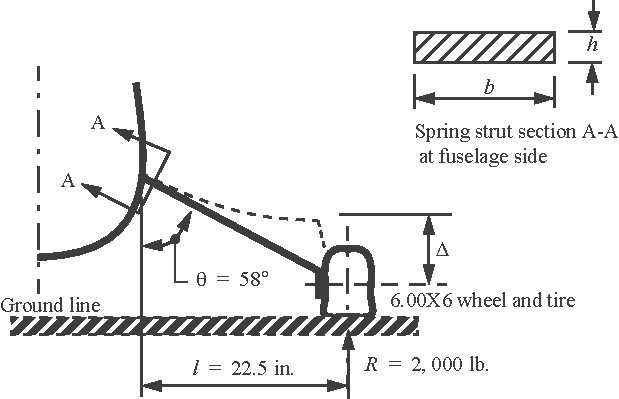
\includegraphics{Figure_14-1.pdf}}
\caption{Sketch of the steel leaf spring strut configuration.\label{fig14.1}}
\end{figure}}

\noindent where $L$ is the length of the strut, $z$ is the axial coordinate; $z=0\ @$ axel, $M_{x}(z)$ is the bending moment, $E$ is Young's modulus, and $I_{x x}$ is the second area moment about the centroidal $x$-axis. Interchanging the derivative and definite integral in eq.~(\ref{eq14.2}), the deflection in the direction of \textit{R} is
\begin{align}\label{eq14.3}
\Delta=\frac{\partial U^{*}}{\partial R}=\int_{0}^{L}\left[\frac{M_{x}}{E I_{x x}} \frac{\partial M_{x}}{\partial R}\right] d z.
\end{align}
To determine how the bending moment, axial force, and shear force depend on \textit{R}, impose static equilibrium conditions on the strut. From the free-body diagram shown in figure~\ref{fig14.2}, we get
\begin{align}\label{eq14.4}
V_{y}+R \sin \theta=0 \quad N+R \cos \theta=0 \quad M_{x}+z R \sin \theta=0 \quad 0 \leq z \leq L.
\end{align}

\vspace*{-1\baselineskip}
{\def\thefigure{14.2}
\processfigure[H]{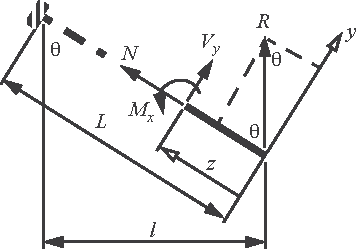
\includegraphics{Figure_14-2.pdf}
}{\caption{Free body diagram of the strut.\label{fig14.2}}}}
\vspace*{-1\baselineskip}

\noindent Substitute the bending moment from eq.~(\ref{eq14.4}) into eq.~(\ref{eq14.3}) to find%\pagebreak
\begin{align}\label{eq14.5}
\Delta=\frac{1}{E I_{x x}} \int_{0}^{L}(-z R \sin \theta)(-z \sin \theta) d z=\frac{R L^{3} \sin ^{2} \theta}{3 E I_{x x}}.
\end{align}
\vspace*{2pt}\vspace*{-8pt}
\pagebreak

\noindent The horizontal length $l=L \sin \theta$. Eliminate strut length in terms of the horizontal length in eq.~(\ref{eq14.5}) to get
\begin{align}\label{eq14.6}
\Delta=\frac{R l^{3}}{3 E I_{x x} \sin \theta}.
\end{align}
Take the strut to be made of steel having a Young's modulus of $30 \times 10^{6}$\,psi. Consider an initial size of
\begin{align}\label{eq14.7}
b=3.0\,\text{in.} \quad h=0.69\,\text{in. }
\end{align}
The cross-sectional area $A=3(0.69)=2.07\,\text{in.}^{2}$. The second area moment about the centroidal $x$-axis in the cross section is
\begin{align}\label{eq14.8}
I_{x x}=\frac{b h^{3}}{12}=\frac{3(0.69)^{3}}{12}=0.0821\,\text{in.}^{4}
\end{align}
Numerical evaluation of the strut deflection is
\begin{align}\label{eq14.9}
\Delta=\frac{(2{,}200\,\mathrm{lb.})(22.5\,\mathrm{in}.)^{3}}{3(30 \times 10^{6}\,\mathrm{lb}./\text{in.}^{2})(0.0821\,\mathrm{in.}^{2}) \sin 58^{\circ}}=4.00\,\mathrm{in.}
\end{align}
The stopping distance $d$ is equal to the stroke of the strut plus the tire deflection. From 6.00X6 tire deflection charts at an inflation pressure of 20\,psi, the tire deflection is 3.14\,in. at 2{,}200\,lb. loading. Hence,
\begin{align}\label{eq14.10}
d=\Delta+3.14\,\text{in.}=7.14\,\text{in.}=0.595\,\mathrm{ft}.
\end{align}

\begin{wrapfigure}[14]{r}{72pt}
\vspace{-19pt}
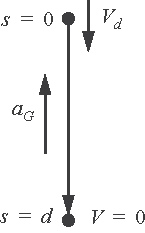
\includegraphics{Figure_14-3.pdf}
\caption{Uniform deceleration along a straight line.\label{fig14.3}}
\end{wrapfigure}

\vspace*{-1pc}

\noindent According to FAR 23.473(d), the initial descent velocity, in feet per second, for landing gear design calculations cannot be less than $4.4(W/S)^{1/4}$, where $W$ is the gross weight in pounds and $S$ is the wing reference area in sq. ft. Assuming $\textit{S} = 157$ ft.$^2$ we get $V_{d}=8.5$ ft./s. Now assume the acceleration of the mass center is constant during the period of landing. Let descent velocity at touchdown be denoted by $V_{d}$, and during the period of landing the vertical speed reduces from $V_{d}$ to zero. The acceleration of the mass center is computed from the uniform acceleration formula given by eq.~(\ref{eq2.14}) on page \pageref{eq2.14}. See figure~\ref{fig14.3}.
\begin{align}\label{eq14.11}
a_{G}=V_{d}^{2} /(2 d)=\frac{(8.5)^{2}}{2(0.595)}=60.714\,\mathrm{ft}/\mathrm{s}^{2}.
\end{align}
The load factor at touchdown is
\begin{align}\label{eq14.12}
n=1+\frac{60.714}{32.2}=2.89.
\end{align}
The load reduction due to wing lift is 0.67 as stipulated in FAR 23.473(e), so the landing gear limit load factor is
\begin{align}\label{eq14.13}
n=2.89-0.67=2.2.
\end{align}

\subsubsection{Strength consideration.} The axial normal stress is due to the superposition of the bending component and the compression component.
\begin{align}\label{eq14.14}
\sigma_{z}=\frac{M_{x} y}{I_{x x}}+\frac{N}{A} \quad-\frac{h}{2} \leq y \leq \frac{h}{2} \quad 0 \leq z \leq L.
\end{align}
Substitute ${M}_x$ and \textit{N} from eq.~(\ref{eq14.4}), and substitute ${I}_{xx}$ from eq.~(\ref{eq14.8}), into eq.~(\ref{eq14.14}) to get
\begin{align}\label{eq14.15}
\sigma_{z}=\frac{-z R \sin \theta(h/2)}{\left(b h^{3}\right)/12}-\frac{R \cos \theta}{b h}=\frac{-6 z R \sin \theta}{b h^{2}}-\frac{R \cos \theta}{b h}.
\end{align}

\vspace*{-1.4pc}

\noindent The axial normal stress (\ref{eq14.15}) attains maximum magnitude at $z = {L}$. For $b = 3$\,in. and $h = 0.69$\,in. the maximum magnitude is
\[
\left.\sigma_{z}\right|_{z=L}=-208{,}503.-563.2=-209{,}066.2\,\mathrm{psi}.
\]
Steel alloy 4340, oil quenched and tempered, has a yield strength of 230 ksi and an ultimate tensile strength of 250 ksi. A major application of alloy 4340 is to aircraft landing gears because of its high strength. For design assume an allowable stress of 160 ksi, which implies a factor of safety of 1.4 with respect to yield. The margin of safety is defined by
\begin{align}\label{eq14.16}
M S=\frac{\text{ excess strength }}{\text{ required strength }}=\frac{\sigma_{\text{allowable }}-\left|\sigma_{z}\right|_{\max }}{\left|\sigma_{z}\right|_{\max }}.
\end{align}
The margin of safety is positive for a feasible design, and negative for an infeasible design. For the design $b = 3$\,in. and $h = 0.69$\,in., the $M S=-0.233$. Therefore, with respect to strength the design (\ref{eq14.7}) is infeasible.

Moreover, the landing gear limit load factor is specified as 2.0 in FAR 23.473(g), and not the 2.2 determined for the initial design (\ref{eq14.7}). To achieve the required landing gear load factor we compute new values for the acceleration, the stopping distance and the stroke of the strut as follows:
\begin{align}\label{eq14.17}
a_{G}=(2-1+0.67) g=53.77\,\mathrm{ft.}/\mathrm{s}^{2} \quad d=V_{d}^{2} /\left(2 a_{G}\right)=8.09\,\mathrm{in}. \quad \Delta=d-3.14=4.95\,\mathrm{in.}
\end{align}
The new second area moment for the leaf spring strut is obtained by a rearrangement of (\ref{eq14.9}):
\begin{align}\label{eq14.18}
I_{x x}=\frac{R l^{3}}{3 E(4.95) \sin \theta}=0.06638\,\text{in.}{}^{4}=\frac{b h^{3}}{12}.
\end{align}
Solve eq.~(\ref{eq14.18}) for $h$ to get
\begin{align}\label{eq14.19}
h=0.9269883/b^{1/3}.
\end{align}
Substitute eq.~(\ref{eq14.19}) for $h$ into axial normal stress (\ref{eq14.15}) and evaluate it at $z = \textit{L}$ to get
\begin{align}\label{eq14.20}
\sigma_{z}=\frac{-1,257.65}{b^{2/3}}-\frac{345,632}{b^{1/3}}.
\end{align}
Set $\left|\sigma_{z}\right|=160{,}000\,\mathrm{psi}$ in eq.~(\ref{eq14.20}), and by a root finding routine, or by a trial and error method, find
\begin{align}\label{eq14.21}
b=10.13\,\text{in.}\qquad h=0.4284\,\text{in. }
\end{align}
For the design (\ref{eq14.21}), the margin of safety (\ref{eq14.16}) is positive for $0 \leq z \leq L$ as shown in figure~\ref{fig14.4}. At $z=L=26.53\,\mathrm{in.}$ it is $6.7 \times 10^{-16} \sim 0$ and at $z = 0$ it is 594.7. The design (\ref{eq14.21}) is feasible with respect to strength and also satisfies the landing gear load factor of 2.

\pagebreak

{\def\thefigure{14.4}
\processfigure{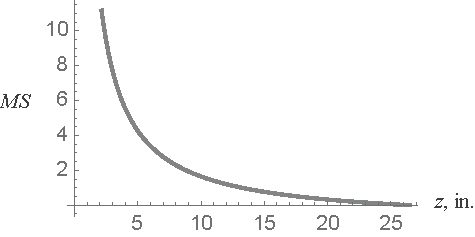
\includegraphics{Figure_14-4.pdf}
}{\caption{Distribution of the margin of safety along the length of the strut for design (\ref{eq14.21}).\label{fig14.4}}}}


\subsection{Strut design exercise}\label{sec14.1.2}

Although the margin of safety is positive along the length of the strut in figure~\ref{fig14.4}, it is very large over most of the length of the strut. An efficient use of material to carry the load has a margin of safety that is sightly positive. The large positive values of the margin of safety shown in figure~\ref{fig14.4} indicate that the design is too heavy. The specific weight of steel is 0.284\,lb./in.$^3$, so the weight of the leaf spring strut (\ref{eq14.21}) is
\begin{align}\label{eq14.22}
W=(0.284\,\mathrm{lb}./\text{in.}^{3})(10.13\,\text{in.})(0.4284\,\text{in.})(26.53\,\text{in.})=32.7\,\mathrm{lb}.
\end{align}
Since the axial normal stress (\ref{eq14.15}) is linear in the coordinate $z$, it is reasonable to assume that the cross-sectional area of the strut should be linear in $z$. Take the thickness of the strut $h$ to be independent of $z$, and let the width of the strut be a linear function of $z$. That is,
\begin{align}\label{eq14.23}
b(z)=b_{L}\left(\frac{z}{L}\right)+b_{0}\left(1-\frac{z}{L}\right) \quad 0 \leq z \leq L,
\end{align}
where $b_{0}$ is the width at the axel and $b_{L}$ is the width at the fuselage. Of course, this means that the second area moment of the cross section, $I_{x x}=\left(b h^{3}\right)/12$, is a linear function of \textit{z}.
\begin{enumerate}
  \item Determine the value of the design variables $h$, $b_{0}$, and $b_{L}$ such that stroke is equal to 4.95\,in. and the magnitude of the normal stress $\sigma_{z}$ is less than, or equal to, an allowable value of 160{,}000\,psi.
  \item Plot the margin of safety for strength of the design in step 1 with respect to $z$ for $0 \leq z \leq L$.
  \item Compute the weight of the design determined in step 1.
\end{enumerate}


\section{Wing spar design}\label{sec14.2}

The wing spar is the primary load bearing structure in the wing. Consider the design of a spar for minimum weight under a particular maneuver condition subject to different design limit states. The example is the Mohawk commuter airplane shown in figure~\ref{fig14.5}. The wing is slightly tapered, but to simplify the analysis we will treat it as uniform. The wing span is 74 feet, and the wing area is 592 square feet, so that the average chord is 8 feet. About 9 feet of this wing span is the fuselage width, so that we will assume that each wing is a 32.5-foot-long cantilever beam. At the root of the wing, the airfoil is NACA 23016, with a thickness-to-chord ratio (\textit{t/c}) of 16 percent, while at the tip, the airfoil is  NACA 32012, with a thickness-to-chord ratio of 12 percent. Assume a constant ${t/c} = 0.14$, corresponding to a maximum thickness of the airfoil of 1.12 ft.

{\def\thefigure{14.5}
\processfigure{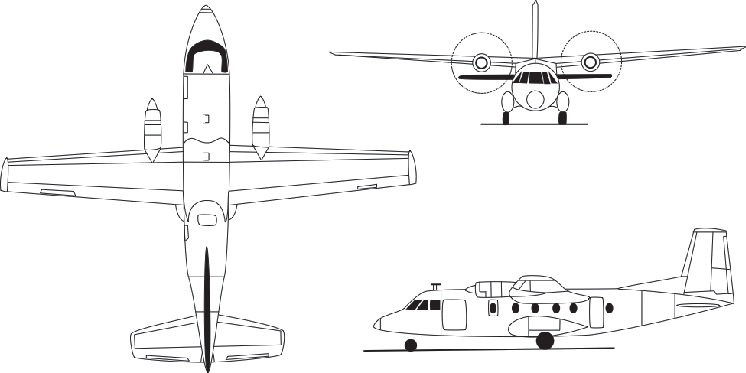
\includegraphics{Figure_14-5.pdf}
}{\caption{Mohawk 298 commuter airplane.\label{fig14.5}}}}


\subsubsection{Design load condition.} The load condition that usually designs most of the wing box is a pull-up maneuver. For transport aircraft the FAA specifies a maneuver of 2.5 g, with a safety factor of 1.5. That is, the wings need to be able to carry about 2.5 times the weight of the airplane without suffering material failure. The maximum takeoff weight is 23{,}810\,lb., but in this condition there is a lot of fuel in the wing, and this fuel provides inertia relief, reducing the stresses in the wing. Also, part of the lift of the wing is provided by the area over the fuselage, so we will assume that the two wings carry 20{,}000\,lb. in cruise, and 50{,}000\,lb. in the design pull-up maneuver.

\subsubsection{Wing box overall dimensions.} Assume a wing box that is 24\,in. in the chord-wise direction and 13\,in. deep so that it can fit into the airfoil. See figure~\ref{fig14.6}.

\vspace*{-1\baselineskip}
{\def\thefigure{14.6}
\processfigure{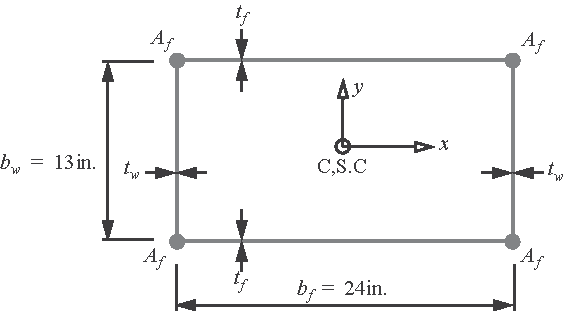
\includegraphics{Figure_14-6.pdf}
}{\caption{Semimonocoque wing\break spar cross section. Design variables are the thicknesses $t_f$ and $t_w$,
and\break the stringer flange area $A_f$.\label{fig14.6}}}}
\vspace*{-0.6\baselineskip}

\subsubsection{Material data.}

1. The wing is made of aluminum alloy 2024-T351 with Young's modulus of $E=10 \times 10^{6}$\,psi, Poisson's ratio of 0.3, a specific weight of 0.1\,lb./in.$^3$, a yield strength in tension or compression of 47{,}000\,psi, and a mode I fracture toughness $K_{I c}=31{,}000\,\mathrm{psi} \sqrt{\mathrm{in.}}$

\subsubsection{Spanwise airload distribution.} Let $z$ denote the spanwise axis along the locus of shear centers of each cross section. The $z$-axis measured from the root to tip, with $0 \leq z \leq z_{\max }$, and
 $z_{\max }=32.5 \times 12=390\,\mathrm{in}.$ Assume that the load is distributed elliptically over the wing as in example \ref{ex6.6} on page \pageref{ex6.6}, so that the load intensity $f_{L}$ per unit span is given as
\begin{align}\label{eq14.24}
f_{L}(\zeta)=\frac{2 L}{\pi z_{max }} \sqrt{1-\zeta^{2}} \quad 0 \leq \zeta \leq 1 \quad \zeta=\frac{z}{z_{max }},
\end{align}
where the total lift $L=50{,}000\,\mathrm{lb.}$, and the wing span $z_{\max }=32.5\,\mathrm{ft.}$

It is given that the line of action of the lift is acting on the front web of the box beam. Equilibrium conditions shown in figure~\ref{fig14.7} determine the shear force, bending moment, and torque at the wing root as

{\def\thefigure{14.7}
\processfigure[!h]{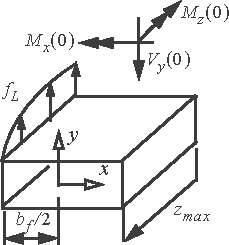
\includegraphics{Figure_14-7.pdf}\raisebox{60pt}{$\begin{array}{@{\hspace*{15pt}}l}-V_y(0)+z_{max}\displaystyle\int\limits_0^1f_L(\zeta)d\zeta=0\\
-M_x(0)-z^2_{max}\displaystyle\int\limits_0^1\zeta f_L(\zeta)d\zeta=0\\
-M_z(0)-\left(\displaystyle\frac{b_f}{2}\right)z_{max}\displaystyle\int\limits_0^1 f_L(\zeta)d\zeta=0\end{array}$}
}{\caption{Free body diagram of~the~spar~and~the equilibrium equations.\label{fig14.7}}}}

\vspace*{-1pc}

\[
V_{y}(0)=\frac{L}{2}=25{,}000\,\mathrm{lb}. \quad M_{x}(0)=\frac{-2 L z_{max }}{3 \pi}=-4.13803 \times 10^{6}\,\mathrm{lb}. \text{-in. } \quad M_{z}(0)=\left(-\frac{b_{f}}{2}\right) \frac{L}{2}=-300{,}000\,\mathrm{lb}.\mbox{-}\mathrm{in}.
\]

\vspace*{-1pc}

\subsection{Evaluation of stresses at root cross section}\label{sec14.2.1}
Since the wing box is uniform along the span, the thicknesses are sized by the conditions at the root. Ten locations for evaluation of the Mises effective stresses and the margins of safety are shown in figure~\ref{fig14.8}.

%{\def\thefigure{14.8}
%\processfigure[H]{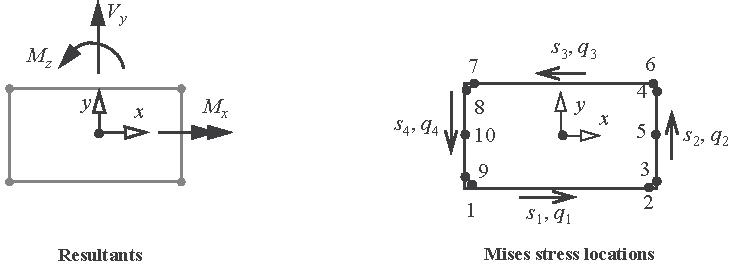
\includegraphics{Figure_14-8.pdf}
%}{\caption{Locations for the evaluation of stresses at the wing root.\label{fig14.8}}}}

{\def\thefigure{14.8}
\begin{figure}[H]
\centering{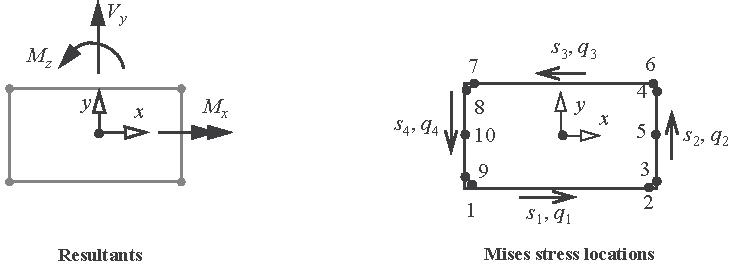
\includegraphics{Figure_14-8.pdf}}
{\caption{Locations for the evaluation of stresses at the wing root.\label{fig14.8}}}
\end{figure}
}

\noindent The axial normal stress at the root due to flexure is determined from eq.~(\ref{eq4.6}) on page \pageref{eq4.6}. For this symmetric cross section we get from eq.~(\ref{eq4.4}) that $n_{x}=n_{y}=0$, $k=1$., and $\bar{y}(s)=y(s)$ by eq.~(\ref{eq4.7}). In the absence of an axial normal force and no thermal loads, the normal stress in eq.~(\ref{eq4.6}) reduces to
\begin{align}\label{eq14.25}
\sigma_{z z}=\frac{M_{x}(0)}{I_{x x}} y(s).
\end{align}
The second area moment about the $x$-axis through the centroid of the cross section is given by
\begin{align}\label{eq14.26}
I_{x x}=A_{f} b_{w}^{2}+(b_f b_{w}^{2} t_{f})/2+(b_{w}^{3} t_{w})/6.
\end{align}
\noindent The shear stresses tangent to the contour are determined from the shear flows and thicknesses of the panels of the box beam (i.e., $\sigma_{z s}=q(s, z)/t(s)$). For the box beam the shear stresses in each branch are
\begin{align}\label{eq14.27}
\left.\sigma_{z s}\right|_{i}=\tau_{i}\left(s_{i}\right)=q_{i}\left(s_{i}\right)/t_{i} \quad i=1,2,3,4,
\end{align}
where $q_{i}\left(s_{i}\right)$ denotes the shear flow in the \textit{i-th} branch, and $s_{i}$ denotes the branch contour coordinate. The total shear flows are the summation of the shear flow due to the transverse shear force acting through the shear center and the torque. From eq.~(\ref{eq4.25}) on page \pageref{eq4.25}, the total shear flow at a given contour location is
\begin{align}\label{eq14.28}
q_{i}\left(s_{i}\right)=\frac{M_{z}(0)}{2 A_{c}}-F_{y}\left(s_{i}\right) V_{y}(0) \quad i=1,2,3,4.
\end{align}
The shear flow distribution function with respect to the shear center $F_{y}(s)$ is obtained from eq.~(\ref{eq4.19}) and eq.~(\ref{eq4.26}), where $x_{sc}=0$. For each branch we write
\begin{align}\label{eq14.29}
F_{y}\left(s_{i}\right)=\frac{1}{I_{x x}}\left[Q_{x i}\left(s_{i}\right)-\frac{1}{2 A_{c}}\left[\oint r_{n} Q_{x} d s\right]\right],
\end{align}
where the area enclosed by the cell $A_{c}=b_f b_{w}$. The functions $Q_{x i}\left(s_{i}\right)$ in eq.~(\ref{eq14.29}) are distribution functions defined by first area moments, and are obtained from eq.~(\ref{eq4.9}) on page \pageref{eq4.9}. For each branch functions $Q_{x i}\left(s_{i}\right)$ are determined from
\[Q_{x 1}\left(s_{1}\right)=\left(\frac{-b_{w}}{2}\right) A_{f}+\int_{0}^{s_{1}} y_{1}\left(s_{1}\right) t_{f} d s_{1},\ Q_{x 2}\left(s_{2}\right)=Q_{x 1}\left(b_{f}\right)+\left(\frac{-b_{w}}{2}\right) A_{f}+\int_{0}^{s_2} y_{2}\left(s_{2}\right) t_{w} d s_{2},\]
\begin{align}\label{eq14.30}
Q_{x 3}\left(s_{3}\right)=Q_{x 2}\left(b_{w}\right)+\left(\frac{b_{w}}{2}\right) A_{f}+\int_{0}^{s_{3}} y_{3}\left(s_{3}\right) t_{f} d s_{3},\ \text{and}\ Q_{x 4}\left(s_{4}\right)=Q_{x 3}\left(b_{f}\right)+\left(\frac{b_{w}}{2}\right) A_{f}+\int_{0}^{s_{4}} y_{4}\left(s_{4}\right) t_{w} d s_{4}.
\end{align}
The contour coordinate functions $[x(s), y(s)]$, functions $Q_{x i}\left(s_{i}\right)$, and the evaluation of coordinates normal to contour $r_{n i}$ are listed in table~\ref{tab14.1}.

\noindent From the results listed in table~\ref{tab14.1}, the integral term on the right-hand side of eq.~(\ref{eq14.29}) evaluates as

\begin{table}[!h]
\processtable{Geometric functions of the contour\label{tab14.1}}{%
\begin{tabular}{@{}llllll@{}}
\toprule
\colhead{Branch} & \colhead{${s}_i$} & \colhead{${x}_i$} &
\colhead{${y}_i$} & \colhead{${Qx}_i$} & \colhead{${r}_{ni},\ \textbf{eq.~(\ref{eq4.11})}$} \\
\midrule
$i =1$ & $0 \leq s_{1} \leq b_{f}$ & $-(b_{f}){/}2+s_{1}$ & $-b_{w}{/}2$ & $(-b_{w} t_{f}s_1){/}2$ & $b_{w}{/}2$\\[3pt]
$i = 2$ & $0 \leq s_{2} \leq b_{w}$ & $b_{f}{/}2$ & $(-b_{w}){/}2+s_{2}$ & $-\frac{b_{f} b_{w} t_{f}}{2}-\frac{b_{w} t_{w} s_{2}}{2}+\frac{t_{w} s_{2}^{2}}{2}$ & $b_{f}{/}2$\\[3pt]
$i = 3$ & $0 \leq s_{3} \leq b_{f}$ & $b_{f}{/}2-s_{3}$ & $b_{w}{/}2$ & $-\frac{b_{f} b_{w} t_{f}}{2}+\frac{b_{w} t_{f}s_{3}}{2}$ & $b_{w}{/}2$\\[3pt]
$i = 4$ & $0 \leq s_{4} \leq b_{w}$ & $(-b_{f}){/}2$ & $b_{w}{/}2-s_{4}$ & $\frac{b_{w} t_{w} s_{4}}{2}-\frac{t_{w} s_{4}^{2}}{2}$ & $b_{f}{/}2$\\[3pt]
\botrule
\end{tabular}}{}
\vspace*{-1pc}
\end{table}

\vspace*{-2pc}

\begin{align}\label{eq14.31}
\frac{1}{2 A_{c}} \oint\left[r_{n} Q_{x}\right] d s=-\left(A_f b_{f} b_{w}^{2}+\frac{b_{f}^{2} b_{w}^{2} t_{f}}{2}\right)/2 b_{f} b_{w}.
\end{align}
The shear flow distribution functions are given in eq.~(\ref{eq14.32}) below.
\begin{align}\label{eq14.32}
\begin{split}
F_{y}\left(s_{1}\right)=\frac{b_{w} t_{f}\left(b_{f}-2 s_{1}\right)}{4 I_{x x}} \qquad F_{y}\left(s_{2}\right)=-\left(\frac{2 A_{f} b_{w}+b_{f} b_{w} t_{f}+2\left(b_{w}-s_{2}\right) s_{2} t_{w}}{4 I_{x x}}\right) \\F_{y}\left(s_{3}\right)=\frac{-b_{w} t_{f}\left(b_{f}-2 s_{3}\right)}{4 I_{x x}} \qquad F_{y}\left(s_{4}\right)=\frac{2 A_{f} b_{w}+b_{f} b_{w} t_{f}+2\left(b_{w}-s_{4}\right) s_{4} t_{w}}{4 I_{x x}}
\end{split}.
\end{align}

\subsubsection{Strength limit state.} The Von Mises criterion given by eq.~(\ref{eq4.31}) on page \pageref{eq4.31} is used to predict the initiation of material yielding. The Mises effective stress is defined by
\begin{align}\label{eq14.33}
\sigma_{\text{Mises }}=\sqrt{\sigma_{z z}^{2}+3 \sigma_{z s}^{2}}.
\end{align}
If $\sigma_{\text{Mises }}<\sigma_{\text{yield }}$, then the material response is elastic, and if $\sigma_{\text{Mises }}=\sigma_{\text{yield }}$ yielding initiates. The margin of safety (\ref{eq14.16}) in this case is
\begin{align}\label{eq14.34}
\textit{MS}=\frac{\sigma_{\text{allowable }}-\sigma_{\text{Mises }}}{\sigma_{\text{Mises }}}=\frac{\sigma_{\text{allowable }}}{\sigma_{\text{Mises }}}-1.
\end{align}
The allowable stress for the strength limit state is the yield strength of the material divided by the factor of safety (FS). That is
\begin{align}\label{eq14.35}
\sigma_{\text{allowable }}=\sigma_{\text{yield }} /(F S).
\end{align}
The margin of safety is nonnegative for a feasible design, otherwise the design is infeasible. It should be zero or a small positive number.


\subsection{Trial design of the monocoque box beam spar}\label{sec14.2.2}
A computer program was written to evaluate the Mises effective stresses at the ten locations of the root cross section using a factor of safety of 1.5. For $t_{f}=0.40\,\mathrm{in.}$, $t_{w}=0.30\,\mathrm{in.}$, and $A_{f}=0$ the weight of the spar is $1{,}053.\mathrm{~lb.}$ The values of the ten margins of safety for this design are listed in table \ref{tab14.2}.

\begin{table}[h]
\processtable{Margins of safety for the trial design\label{tab14.2}}{%
\tabcolsep=30pt\begin{tabular}{@{}ll|ll@{}}
\toprule\\[-15.5pt]
& & & \\[-6pt]
MS$_1$ & 0.0528 & MS$_6$ & 0.0714\\
MS$_2$ & 0.0714 & MS$_7$ & 0.0528\\
MS$_3$ & 0.0702 & MS$_8$ & 0.0378\\
MS$_4$ & 0.0702 & MS$_9$ & 0.0378\\
MS$_5$ & 9.086 & MS$_{10}$ & 2.619\\[-8pt]
& & \\[-3.5pt]
\botrule
\end{tabular}}{}
\vspace*{-18pt}
\end{table}

\noindent Since the margins of safety are all positive, this design is feasible. Although feasible, this design is too heavy and, consequently, not optimal. Lower weight feasible designs will have a nonnegative minimum margin of safety close to zero.

To aid in the search for the best design, consider the design plane shown in figure~\ref{fig14.9}. The thickness $t_f$ is the abscissa and the thickness $t_w$ is the ordinate. Each point in the plane represents a design, some are feasible some are not. Contours of constant margins of safety and constant spar weights are plotted in the design plane\footnote{Fig.~\ref{fig14.9} was generated by the \textit{Mathematica} function \textbf{ContourPlot[Min[MS[tf,tw,0]] == 0, \{tf, 0.3, 0.8\},\{tw, 0.0, 0.3\}]}, where definition of function \textbf{MS[tf,tw,Af]} is determined by eq. (\ref{eq14.34}) and the ten points shown in figure~\ref{fig14.8}.}. Only designs with a nonnegative margin of safety are feasible. The least weight design occurs at a point $\left(t_{f}^{*}, t_{w}^{*}\right)$ on the margin of safety contour equal to zero. A second condition is needed to determine point $\left(t_{f}^{*}, t_{w}^{*}\right)$. This second condition is to equate the slope $t_{w}/t_{f}=-\left(\frac{\partial M S}{\partial t_{f}}\right)/\frac{\partial M S}{\partial t_{w}}$ on the margin of safety contour $M S=0$ to the slope of the constant weight contour $t_{w}/t_{f}=(-b_{f})/b_{w}$. That is, the point $\left(t_{f}^{*}, t_{w}^{*}\right)$ on the contour $M S=0$ is tangent to the contour of least weight.




\subsection{Design exercise A}\label{sec14.2.3}

Write a computer program to find the thicknesses ${t_f}$ and ${t_w}$ of the wing box for $A_{f}=0$ that will minimize the weight and carry the load without experiencing material yield using a factor of safety of 1.5. Calculate the weight of the spar and the margins of safety at the ten locations shown in figure~\ref{fig14.8}. Although the design given in article \ref{sec14.2.2} is too heavy, it can be used to assess if the computer program is correct. Include a print out of the program and the output for the best design, which includes the ten margins of safety and the weight.

{\def\thefigure{14.9}
\processfigure[t]{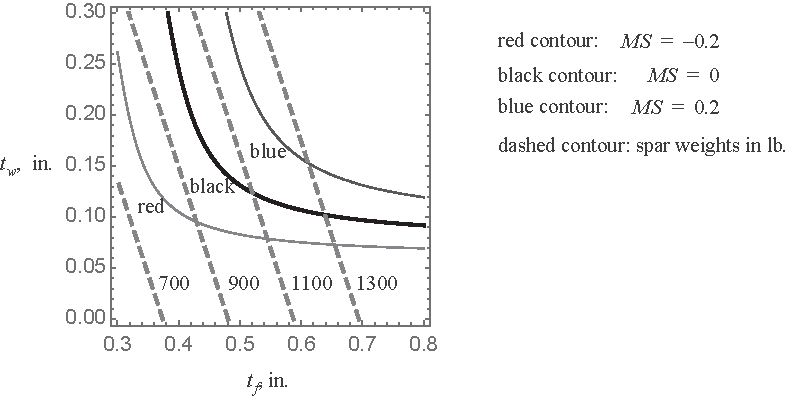
\includegraphics{Figure_14-9.pdf}
}{\caption{Design plane for ${\textbf{\textit{A}}}_{\textbf{\textit{f}}} \boldsymbol{=} \textbf{0}$.
Contours of the margin of safety for yield
and contours of constant spar weights.\label{fig14.9}}}}


\section{Additional limit states for buckling and fracture}\label{sec14.3}

Consider design variables $t_{f}>0$, $t_{w}>0$, and $A_{f} \geq 0$ for the Mohawk 298 wing spar subject to constraints on yielding, buckling, and fracture. The locations in the cross section at the wing root where the design constraints are evaluated are shown in figure~\ref{fig14.10}.

{\def\thefigure{14.10}
\processfigure{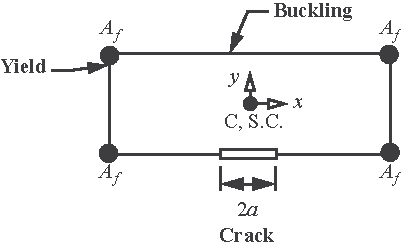
\includegraphics{Figure_14-10.pdf}
}{\caption{Cross section of the stringer-stiffened box beam, and locations of constraint evaluations.\label{fig14.10}}}}


\subsection{Buckling margin of safety}\label{sec14.3.1}

Let rib spacing along the span, or $z$-axis, at the root of the wing be denoted by $a_{1}$, and take $a_{r}=b_{f}/2$. The upper cover skin, or branch 3 with coordinates $[x_{3}(s_{3}), y_{3}]$, is subject to compression and shear. The normal stress is $\sigma_{z z}=\left(M_{x} y_{3}\right)/I_{x x}$ and the shear stress $\tau_{3}\left(s_{3}\right)$ is a linear function in the contour coordinate $s_3$. Assume the skin can be modeled as simply supported flat plate between stiffeners for the buckling analysis. From eq.~(\ref{eq11.118}) on page \pageref{eq11.118} the combined compression and shear index for buckling is defined by
\begin{align}\label{eq14.36}
f_{b}=\left(\frac{\tau_{\text{ave }}}{\tau_{\mathrm{cr}}}\right)^{2}+\left(\frac{\left|\sigma_{z}\right|}{\sigma_{\mathrm{cr}}}\right),
\end{align}
where $0 \leq f_{b}<1$ for no buckling and $f_{b}=1$ at the onset of buckling. The average shear stress is
\begin{align}\label{eq14.37}
\tau_{\text{ave }}=\left(\frac{1}{b_f}\right) \int_{0}^{b_{f}} \tau_{3}\left(s_{3}\right) d s_{3}.
\end{align}
The critical stresses for compression (\ref{eq11.110}) and shear (\ref{eq11.116}) are
\begin{align}\label{eq14.38}
\sigma_{c r}=k_{c} \frac{\pi^{2} E}{12\left(1-v^{2}\right)}\left(\frac{t_{f}}{b_f}\right)^{2} \quad \tau_{\mathrm{cr}}=k_{s} \frac{\pi^{2} E}{12\left(1-v^{2}\right)}\left(\frac{t_{f}}{b_f}\right)^{2}.
\end{align}
The buckling coefficients are
\begin{align}\label{eq14.39}
k_{c}=\left(\frac{1}{\left(a_{r}/b_{f}\right)}+\left(\frac{a_{r}}{b_{f}}\right)\right)^{2}=6.25 \quad k_{s}=4.22565+\frac{5.19931}{a_{r}/b_{f}}=14.624.
\end{align}
The margin of for the buckling limit state is
\begin{align}\label{eq14.40}
M S_{b}=\frac{1-f_{b}}{f_{b}}.
\end{align}

\subsection{Fracture margin of safety}\label{sec14.3.2}

The design damage condition is a through crack centered in the lower left skin that is 1.00\,in. long ($2 a=1.00\,\mathrm{in} $.) with the crack faces perpendicular to the $z$-axis. The lower skin, or branch 1 with coordinates $\left[x_{1}\left(s_{1}\right), y_{1}\right]$, is subject to a tensile stress $\sigma_{z z}=\left(M_{x} y_{1}\right)/I_{x x}$ and a shear stress $\tau_{1}\left(s_{1}\right)$ that is a linear function of contour coordinate $s_1$. Thus, the crack is exposed to tension and shear, which leads to mixed mode cracking (i.e., a mixture of mode I and mode II). The stress intensity factor for mode I is $K_{I}=\sigma_{z z} \sqrt{\pi a}$, and the stress intensity factor for mode II is $K_{I I}=\tau_{1} \sqrt{\pi a}$. The fracture toughness for mode I loading only is $K_{I c}$, and the fracture toughness for mode II loading only is $K_{I I c}$. A fracture criterion for mixed mode loading is given by eq.~(\ref{eq13.42}) on page \pageref{eq13.42}. The plane strain fracture toughness for mode I loading is usually readily available in the literature, but the mode II fracture toughness is not usually available. Tests for mode II are more difficult to design than for mode I. Usually mode II loading does not lead to fracture (Anderson, 1995)\footnote{Mode II loading is important if there is weak interface in the material, which is the case for delamination of filamentary composites as discussed in article \ref{sec13.7} on page \pageref{sec13.7}.}. In other words $K_{I I c}>K_{I c}$. In addition for the design\break $(t_{f}, t_{w}, A_{f})=(0.4,0.3,0)$, the stresses at the center of branch 1 are $\sigma_{z z}=29{,}202.8\,\mathrm{psi}$ and $\tau_{3}\left(b_{f}/2\right)=-1{,}201.92\,\mathrm{psi}$. The shear stress is about 4 percent of the normal stress, and so it is expected that shear would have a small influence on fracture. Thus, we assume fracture is in mode I. The margin of safety for fracture is
\begin{align}\label{eq14.41}
M S_{f}=\frac{K_{I c} /\left(F S_{f}\right)-K_{I}}{K_{I}},
\end{align}
where the factor of safety for fracture is specified as $F S_{f}=1.2$.


\subsection{Design exercise B}\label{sec14.3.3}

Consider a longitudinally stiffened configuration of the wing box for the Mohawk 298 commuter airplane described in article \ref{sec14.3}. Write a computer program to determine the thicknesses $t_{f}$ and $t_{w}$ of the wing box for selected values of the flange area $A_{f}$ listed in the table below. The objective is to minimize the weight. The design limit states are material yield (\ref{eq14.34}) using a factor of safety of 1.5, that the compression panel of the upper skin does not buckle (\ref{eq14.40}), and that the crack in the lower panel does not propagate (\ref{eq14.41}). Evaluate the margin of safety for yield at point 8 shown in figure~\ref{fig14.8}. The minimum margin of safety should not be negative for a feasible design, but should be a small positive number. Write a computer program to determine the thicknesses $t_{f}$ and $t_{w}$ of the wing box for selected values of the flange area $A_{f}$ listed in table \ref{tab14.3}.

\begin{table}[h]
\processtable{Design exercise B\label{tab14.3}}{%
\begin{tabular}{@{}lllllll@{}}
\toprule
& & & & \multicolumn{3}{c}{\colhead{Margins of safety}}\\[-6pt]
& & & & \multicolumn{3}{c@{}}{\hrulefill}\\
\colhead{$A_{f}$, in.$^\textbf{2}$} &  \colhead{$t_{f}$, in.} & \colhead{$t_{w}$, in.} & \colhead{weight, lb.} & \colhead{Yield} & \colhead{Buckling} & \colhead{Fracture}\\
\midrule
0 & \multicolumn{6}{c}{}\\
1.0 & \multicolumn{6}{c}{}\\
2.0 & \multicolumn{6}{c}{}\\
3.0 & \multicolumn{6}{c}{}\\
\botrule
\end{tabular}}{}
\end{table}

\vspace*{-15pt}

\begin{thebibliography}{}\label{sec14.4}
\bibitem{}
Anderson, T.L. \textit{\textbf{Fracture Mechanics}}, 2d ed. Boca Raton, FL: CRC Press Inc., 1995, p. 87.

\bibitem{}
Dowling, N. \textit{\textbf{Mechanical Behavior of Materials}}. Englewood Cliffs, NJ: Prentice-Hall, Inc., 1993, pp. 245--252.

\bibitem{}
Thurston, David B. \textbf{\textit{Design For Flying}}. 2d ed. New York: TAB Books, a Division of McGraw-Hill, Inc., 1995, pp.~237--245.
\end{thebibliography}


\end{document} 